

Most analysis of t-SNE, including the previous section, is concerned with whether it faithfully depicts global structure, specifically cluster structure. In this section, we consider how t-SNE represents points that drastically deviate from the global structure: namely, outliers. It is natural to hope that data visualization methods can enable the identification of outliers. Unfortunately, we find that t-SNE may arbitrarily suppress the severity of outliers present in the input dataset.
%The previous section studied that t-SNE is invariant under certain \textit{global} transformations of the input dataset. This 


%In particular, we prove that stationary t-SNE plots are liable to dramatically misrepresent the structure of data when it comes to \textit{outliers}, i.e. points lying significantly far away from the rest of the point cloud. {\color{red} Strengthen the above and give more introduction before u start explaining what is going on.}
%One of the difficult truths of studying real-world data is the presence of outliers, i.e.\ data points which do not conform to the behavior of the bulk of the data. Geometrically, one can define an outlier as a point lying significantly far away from the rest of the point cloud. It is natural to hope that data visualization techniques would visualize outliers as such.

This phenomenon has been observed empirically in prior work, though  to our knowledge we are the first to formalize it \citep{Schubert2017}. An intuitive explanation of t-SNE's response to outliers can be made based on the asymmetry of the input and output affinity matrices of t-SNE. Roughly speaking, the input affinity behaves like a normalized, symmetrized nearest neighbor graph, whereas the output affinity behaves more like a radius neighbors graph. This means the output affinity is optimized to represent the outlier point in close proximity with at least some points, even if it was extremely far from those points in the input. %This means the input affinity records an outlier–––even a very extreme one–––as having some set of neighbors. The output affinity is optimized to respect this, and hence places the outlier close to some points. 

To begin to formalize this observation, we provide a geometric definition of an outlier.

\begin{definition}\label{def:alpha_outlier}%(\(\alpha\)-outlier configuration) 
Fix \(X \subset \mathbb{R}^D\) %, \textcolor{red}{\(x_0\in X\)}, 
and \(\alpha \in \mathbb{R}_{\geq 0}\). We say \(X\) is an \textbf{\((\alpha, x_0)\)-outlier configuration} if there exists a hyperplane separating \(x_0\) and \(X\setminus \{x_0\}\) 
with margin width at least
   \begin{equation*}\label{eq:alpha_margin}
       \alpha \cdot \max\{1, \diam(X\setminus\{x_0\}) \}.
   \end{equation*}
%i.e., there exists a unit vector \(v \in \mathbb{R}^D\) such that for all \(x\in X\setminus\{x_0\}\), \((v-x_0)\cdot (x-x_0)\) is at least the above.  
  % \textcolor{red}{use max}
   %\textcolor{red}{do a plus 1. this will make the proof much easier. avoids issues with diameter = 0.}
 Define the \textbf{outlier number} of a dataset%\todo{Measure might be an overloaded word in a math context?}
 , denoted \(\alpha(X)\), as the largest \(\alpha\) for which there exists \(x_0 \in X\) such that \(X\) is an \((\alpha, x_0)\)-outlier configuration.
\end{definition}



This definition can be generalized to accommodate more than one outlier. Note that \(\alpha\) is defined with respect to a \textit{thresholded} data diameter\footnote{The choice of a fixed threshold is arbitrary and does not meaningfully affect the results.}, i.e.\ \(\max\{1,\diam(X\setminus\{x_0\})\}\), to maintain a suitable notion of an outlier even in the extreme case of \(\diam(X\setminus\{x_0\}) = 0\). 
%{Note that the outlier extremity \(\alpha\) is defined relative to the diameter of the rest of the points. If the diameter is below a threshold, we resort to an additive definition of outlier extremity.} While the particular threshold is arbitrary, the choice of a threshold is important as it allows us to have a suitable notion of outlier in extreme cases such as when \(\diam(X\setminus\{x_0\}) = 0\). 

%The choice of a threshold here is important and intuitive: it allows us to have a suitable notion of outlier in extreme cases such as when \(\diam(X\setminus\{x_0\}) = 0\).



Our main theorem establishes that any stationary t-SNE output, \textit{regardless of its input}, is incapable of depicting extreme outliers. %, in the sense that the \(\alpha\) number is bounded by a small constant. %, in the sense that the \(\alpha\) outlier measure of any stationary t-SNE output is upper-bounded by a small universal constant. %We show this by analyzing the gradient on the outlier point. The following lemma will be useful. %For simplicity, we work in one dimension, and we make the assumption that





\begin{figure}[t!]
    \centering
%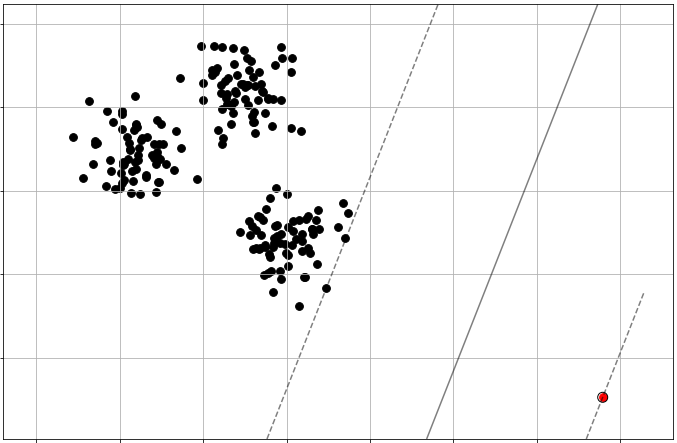
\includegraphics[width=0.49\linewidth]{./images/outlier_figs/illustrative_plot_.png}
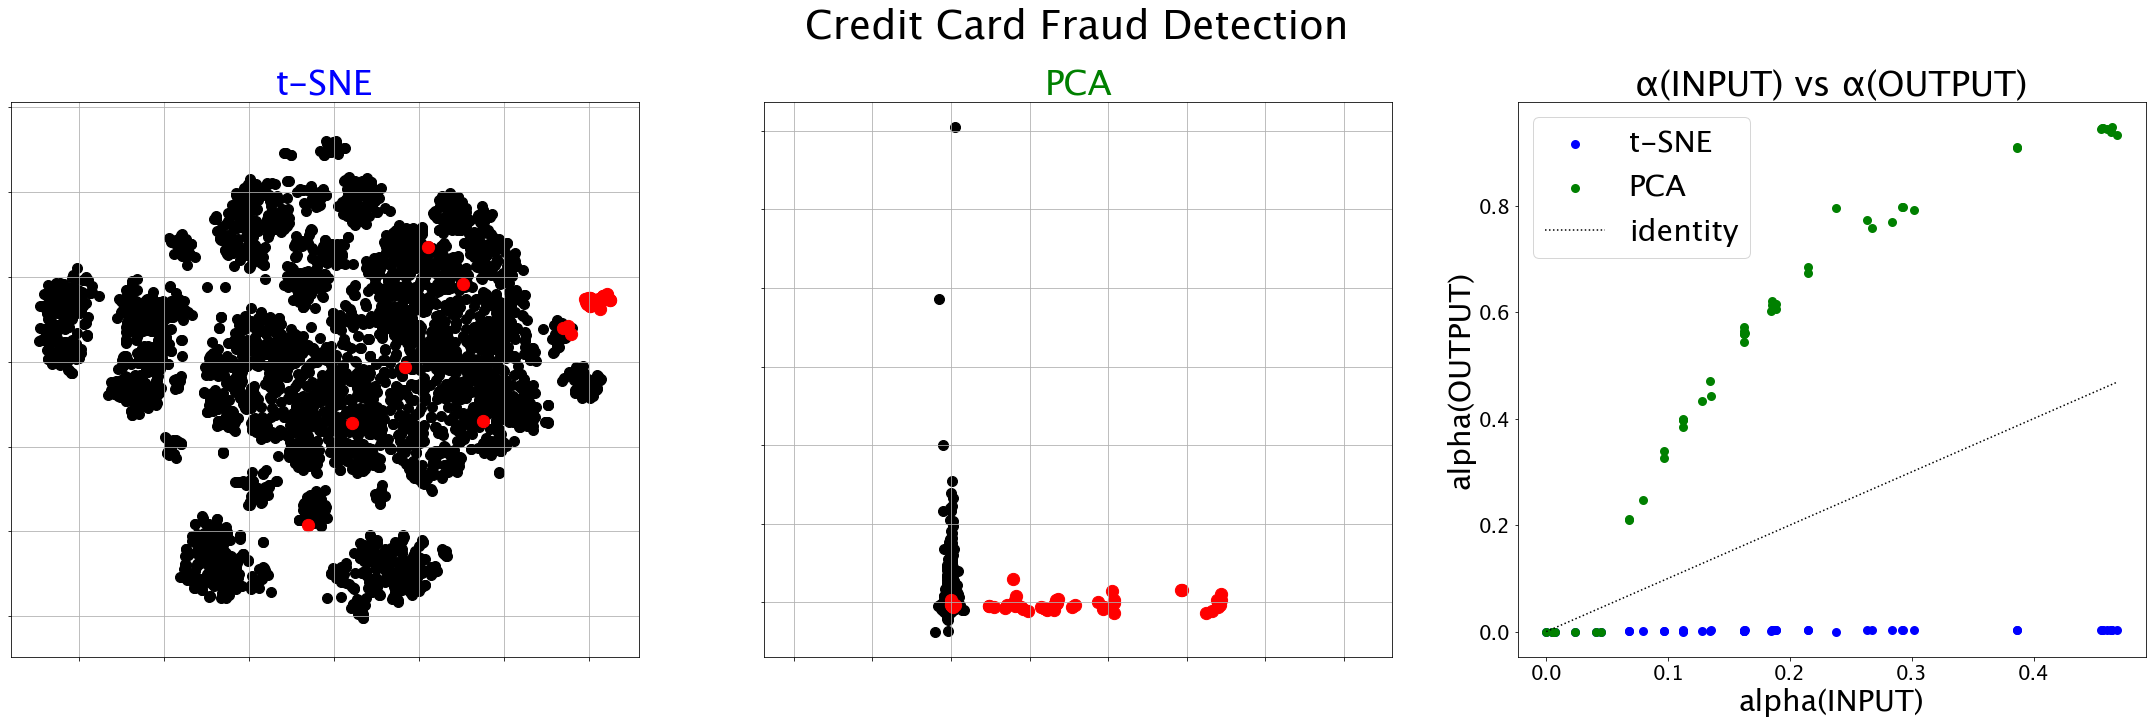
\includegraphics[width=\linewidth]{./images/outlier_figs/credit_card_full.png}
          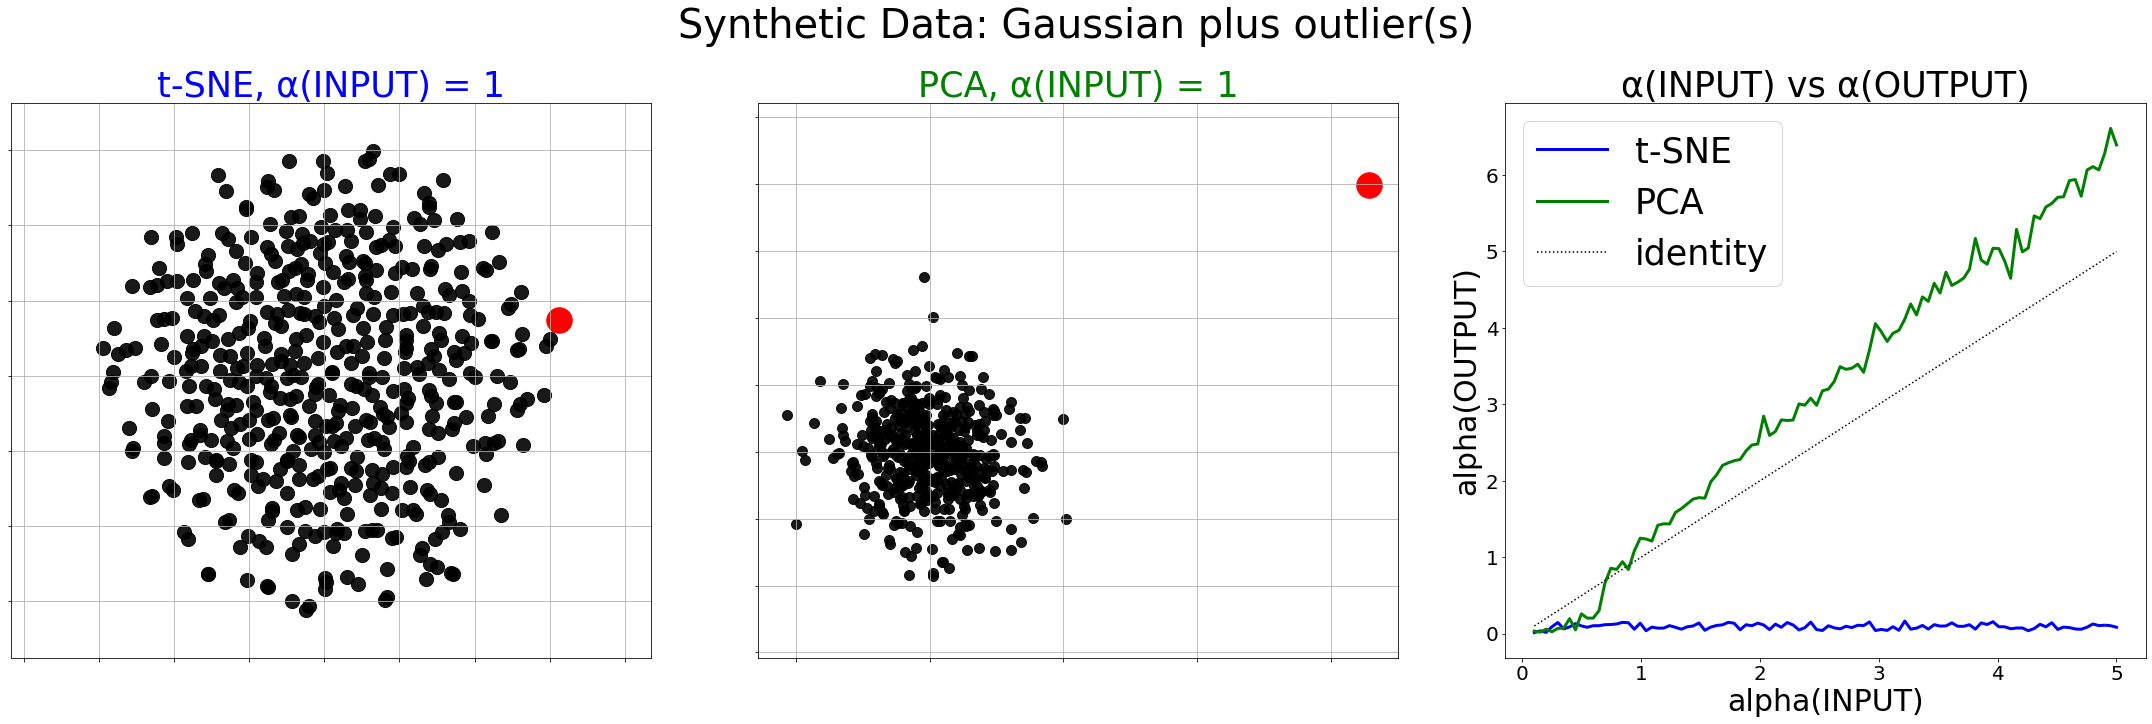
\includegraphics[width=\linewidth]{./images/outlier_figs/OUTLIER_MAIN1.png}
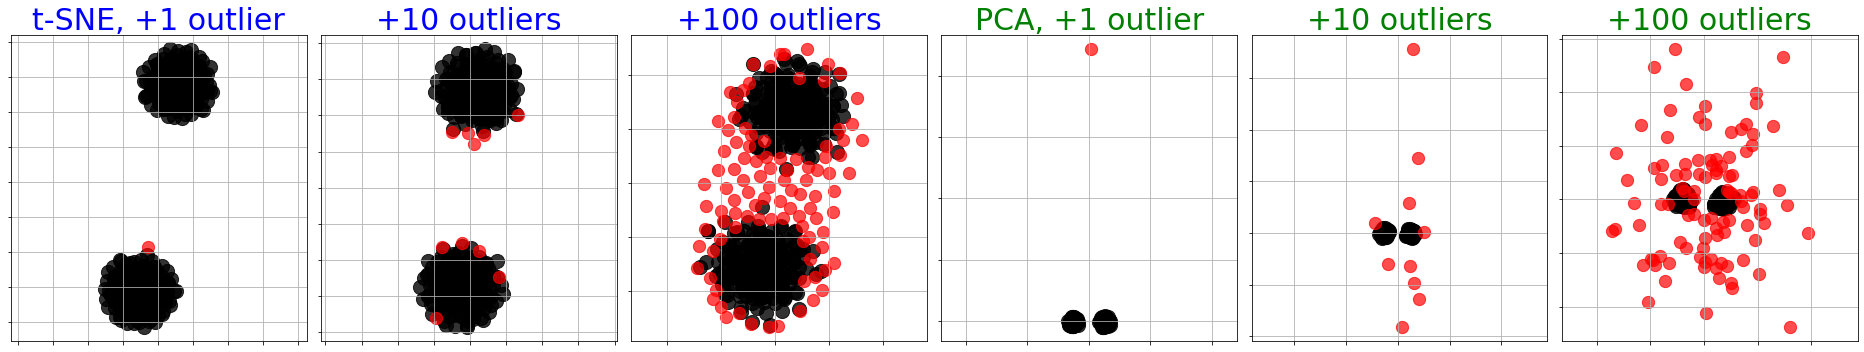
\includegraphics[width=\linewidth]{./images/outlier_figs/OUTLIER_MAIN2.png}
%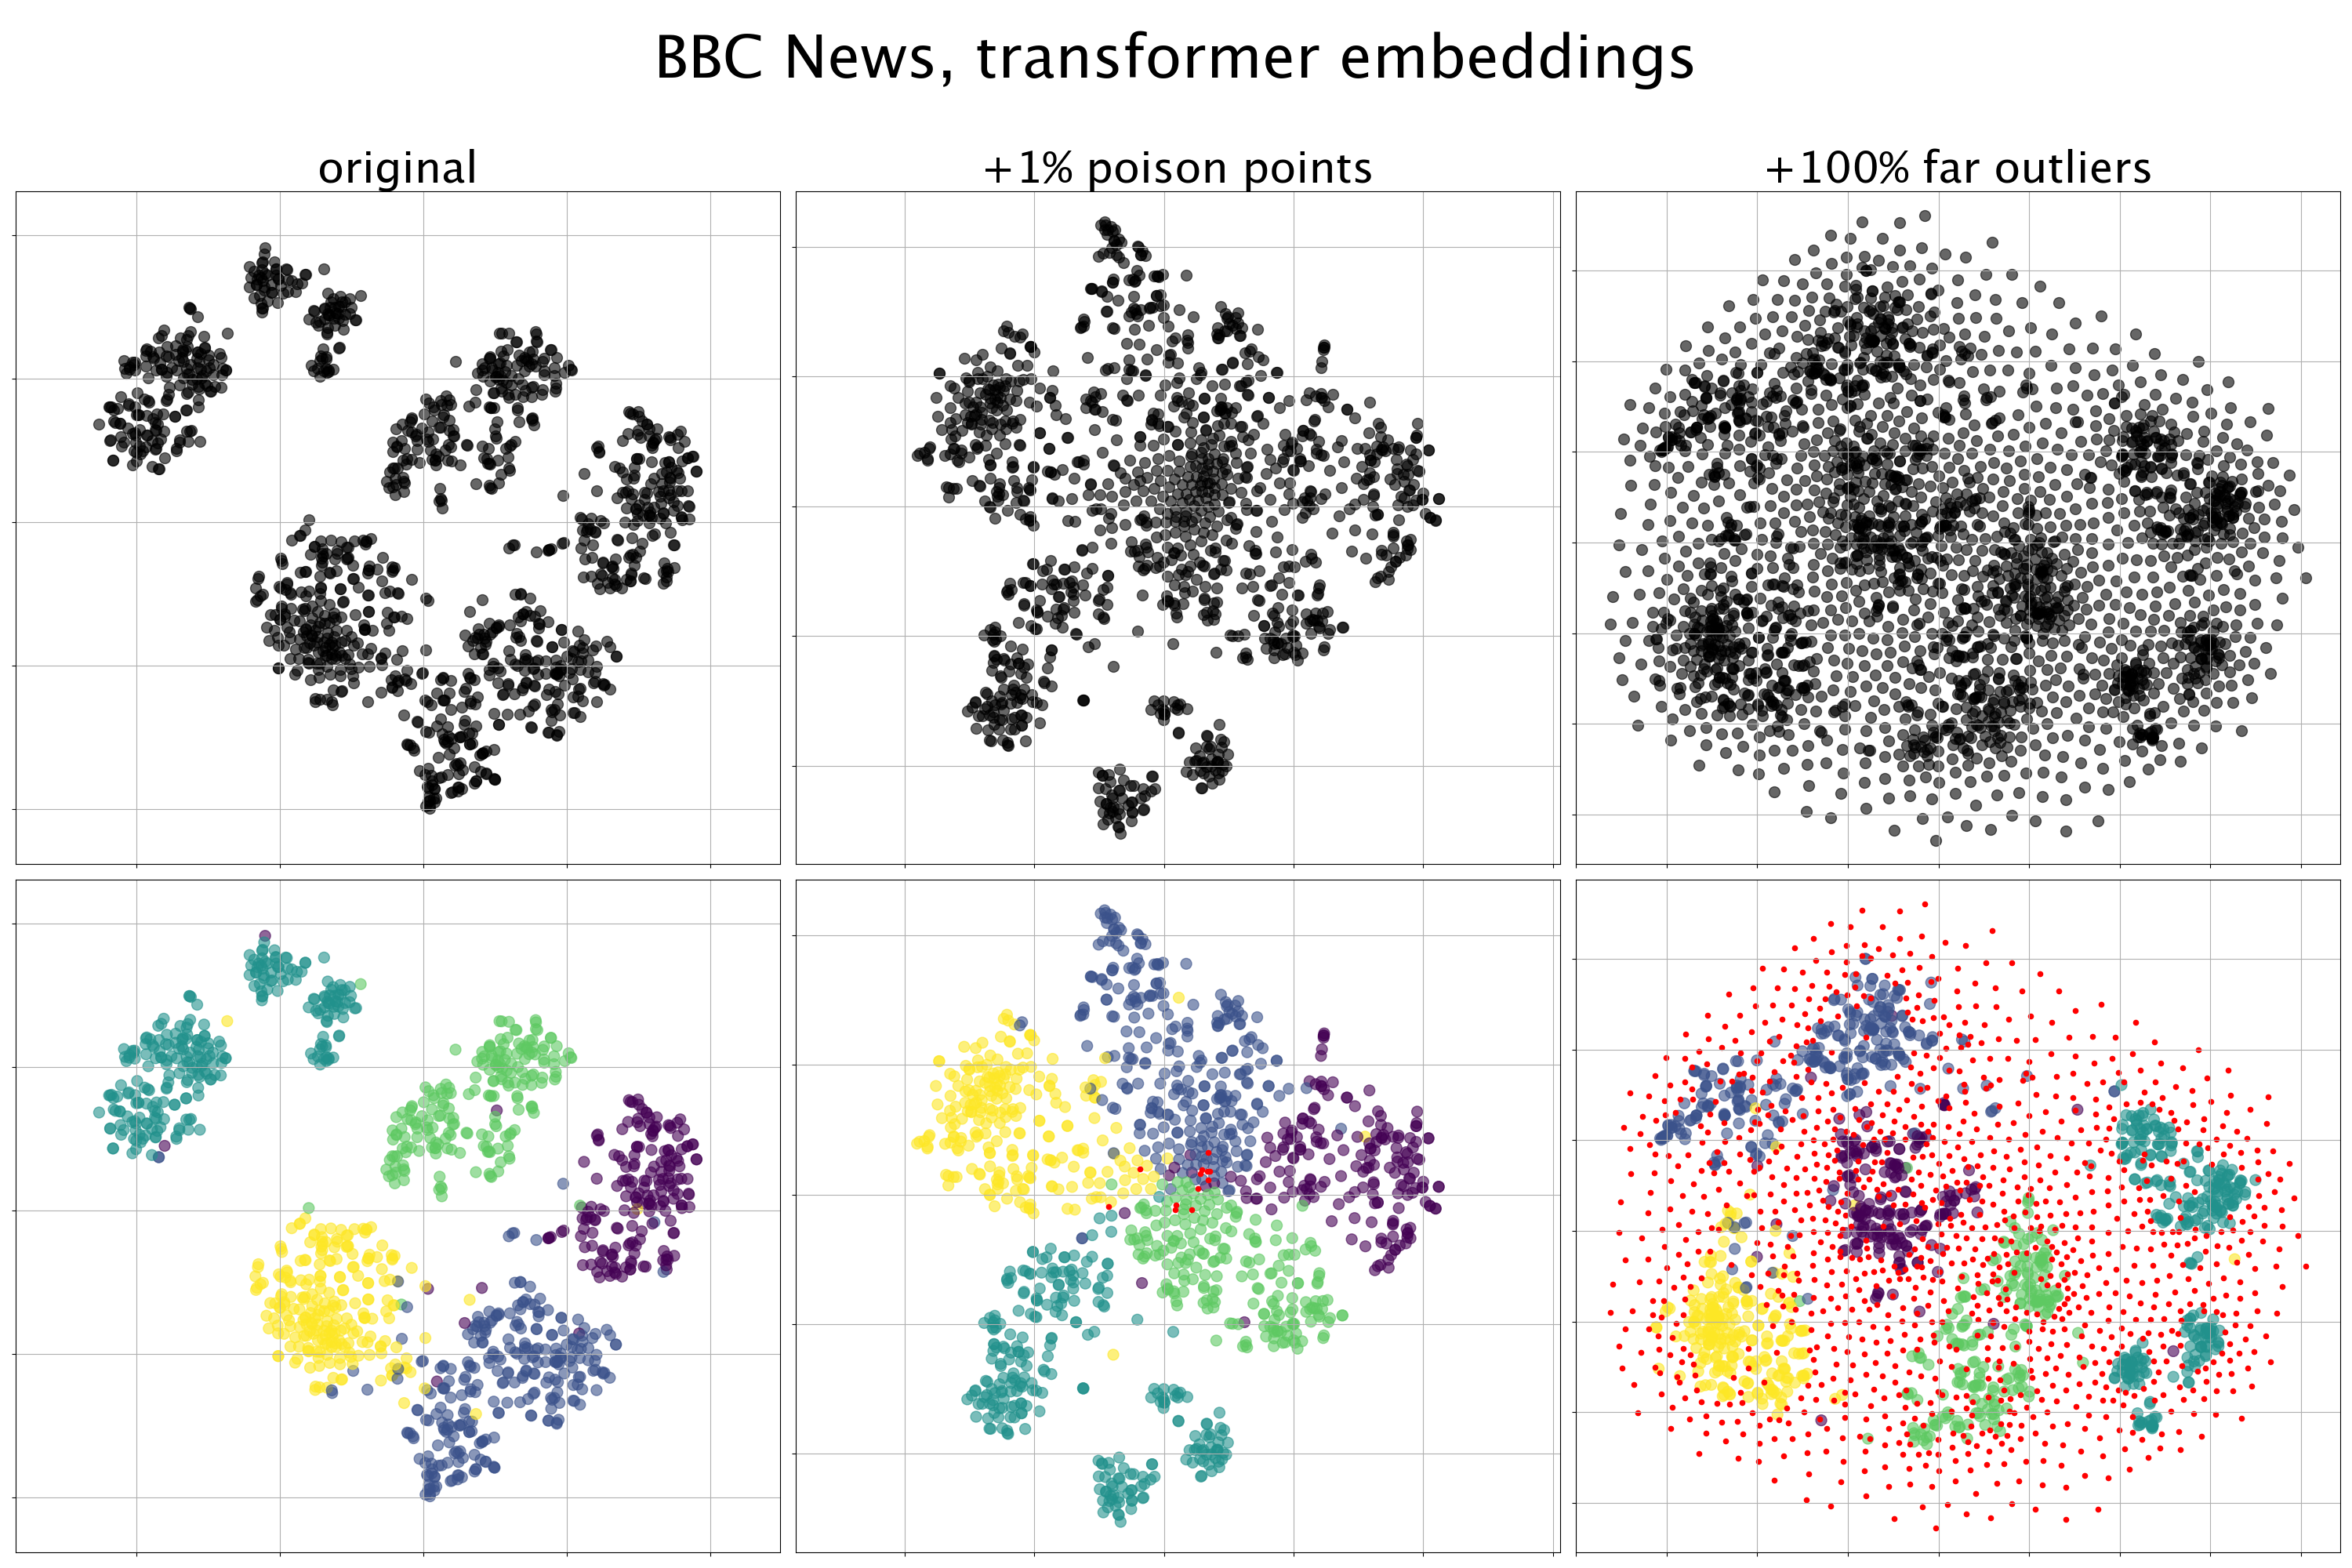
\includegraphics[width=0.707\linewidth]{./images/outlier_figs/OUTLIER_REAL2.png}
%\vspace{-0.2in}
    \caption{
    \small
    t-SNE's response to \(\alpha\)-outliers, compared with PCA. Top row: given data monitoring financial activity (\(n=5050\), \(D=30\)) where one percent of users are committing fraud, PCA succeeds and t-SNE fails at representing the fraudulent users as outliers. Note that all of the fraudulent users register as \((\alpha > 0)\)-outliers with respect to the regular users; in the top right we show how t-SNE and PCA represent those \(\alpha\)-values in their output. Middle row: a similar analysis on a synthetic dataset comprised of a Gaussian sample plus an outlier. Bottom row: mixture of two Gaussians plus 1, 10, and 100 outliers. t-SNE shows the outliers are essentially part of the cluster structure, while for PCA the outliers overtake the structure of the embedding. %In the top row, we compare t-SNE and PCA's visualization of a dataset regarding credit card fraud detection; in particular, we plot \(\alpha(X,x_0)\). In the middle row, we run a similar analysis on a synthetic data model of a set of Gaussian samples plus an outlier. 
    } 
    \label{fig:outliers1}
    %\vspace{-0.15in}
\end{figure}

\begin{restatable}{theorem}{OutlierAbs} 
\label{thm:outlier_abs}
Fix \(n > 2\) %\todo{$n\geq 2$ otherwise $\rho$ is not defined.} we're actually woprking with n+1 points, so I updated rho. 
and \(\rho \in [1,n-1]\). Let \(Y \in {\IMTSNE} \) be \emph{any} stationary t-SNE embedding. Then we have:
\[\alpha(Y) \leq %\sqrt{1 + \Big(1 + \frac{2}{n-2}\Big) \Big(\frac{\textcolor{red}{12}}{1 + \sum_{i=1}^{n-1} P_{0|i}(X)}\Big)} = 
%\sqrt{13 + \frac{24}{n-2}} = 3.606 + o_n(1).\]
3.266 + o_n(1).\]


%for all \(X = \{x_0, x_1,\ldots,x_{n-1}\}\) such that \(Y\in \TSNE_{\rho}(X)\).
%and \(\rho \in [1,n]\). Let \(Y = \{y_0, y_1,\ldots,y_{n}\} \in {\IMTSNE} \) be a stationary t-SNE embedding. Without loss of generality let \(y_0\) be the outlier point. Then we have:
%\[\alpha(Y) = \alpha(Y,y_0) \leq \sqrt{1 + \Big(1 + \frac{2}{n-1}\Big) \Big(\frac{8}{1 + \sum_{i=1}^n P_{0|i}}\Big)} = 3 + o_n(1)\]
%for all \(P(X) = P(\{x_1,\ldots,x_n\})\) such that \(Y\in \TSNE_{\rho}(X)\).
\end{restatable}
%\todo[inline]{why does X even need to be instantiated? Can't we use the 'best' X and make it completely disappear? also "= 3.602+0(1)" (the equals sign) seems a bit funny (i know it is correct)}
The result is proven via analysis of the t-SNE gradient: we argue that if the outlier is too far away, its gradient is nonzero, thus violating stationarity. Key to this analysis is a comparison between the aggregate behavior of the outlier point's affinities in the input versus the output; in other words, the comparison between \(\sum_{i=1}^n P_{i0}\) and \(\sum_{i=1}^n Q_{i0}\). This is where the fundamental asymmetry of t-SNE comes in. While the latter is dependent on the position of the outlier point \(y_0\), per Lemma \ref{lem:Qsum_bound}, the former has a lower bound of \(1/(2n)\) due to the normalization of the conditional affinity probabilities. 
%The key fact behind this result is the normalization of the \(P\) matrix. 


The input-agnostic nature of this result is striking: even if the input is an extreme outlier configuration, no stationary t-SNE output can depict its extremity past roughly \(\alpha \approx 3.6\). This behavior stands in stark contrast to that of principal component analysis (PCA), as shown in Figure \ref{fig:outliers1} on both real and synthetic data models. PCA tends to roughly preserve the \(\alpha\) outlier number, while t-SNE seldom depicts outliers past \(\alpha > 0.2\) in practice, and sometimes even depicts them as within the convex hull of the rest of the points (yielding \(\alpha = 0\)). Furthermore, when faced with multiple outliers, (Figure \ref{fig:outliers1}, bottom) t-SNE gracefully accommodates them into the global structure of the bulk of the data, in contrast to PCA, which depicts the outliers as randomly scattered. %We make this comparison in practice, where we find, somewhat strikingly, that \(\alpha\) tends to hover quite close to \(0\). Visually, in the plots, outliers are often unnoticeable. %The values of \(\alpha\) we observe from t-SNE outputs hover well below \(1\)

Our result suggests that t-SNE is the wrong tool to use in situations involving outlier detection. Consider, for instance, a dataset of financial transactions where the goal is to detect fraudulent users, studied by \citet{dalpozzolo2015_calib}. In this dataset, only \(0.172\)\% percent of the points ($492$ out of $284,807$) are fraudulent and by many standard statistical metrics register as outliers. Comparing the t-SNE and PCA plots on a  random representative subset of this data ($5050$ points, of which $50$ are fraudulent), we see that t-SNE mixes the frauds with the bulk of the points %hides \textcolor{red}{mixes?} the frauds
while PCA keeps them separated for the most part%depicts most of them as far away \textcolor{red}{keeps them separated?}
, see Figure \ref{fig:outliers1}, top row.

Finally, note the distinction between t-SNE's muted response to outliers and its dramatic sensitivity to poison points. We illustrate this distinction on a dataset of BBC news articles which cluster into five topics \citep{bbc_dataset}, see Figure \ref{fig:outliers_real_world}. Given RoBERTa \citep{liu2019roberta} sentence embeddings of these articles (\(n=2225, D=1024\)), we find that injecting $220$ poison points, i.e.\ roughly 10\% (see Appendix \ref{sec:appendix_outliers_experiment} for the explicit construction) can halve the silhouette score of the t-SNE embedding with respect to the ground-truth labelling, whereas injecting $1100$, i.e.\ roughly 50\%, $\alpha$-outliers for $\alpha \in (0.8,1)$ does not degrade the cluster structure. %\blue{COMPUTE ALPHAS} %\textcolor{blue}{unclear why highlight that 1100 outliers improves sil score? worth including what is the min alpha value? perhaps data construction in appendix?} %Figure \ref{fig:bbc_appendix}.%\textcolor{red}{refer to fig 5? cite bbc dataset?}


%\begin{theorem}
 %   For all \(\alpha> 1\), there exists a perplexity \(\rho\) and a dataset \(X_\alpha\) which is an \((\alpha, x_0)\)-outlier configuration with affinity matrix \( P=P_\rho(X_\alpha)\) such that    \[\]
%\end{theorem}




\begin{figure}
    \centering
  %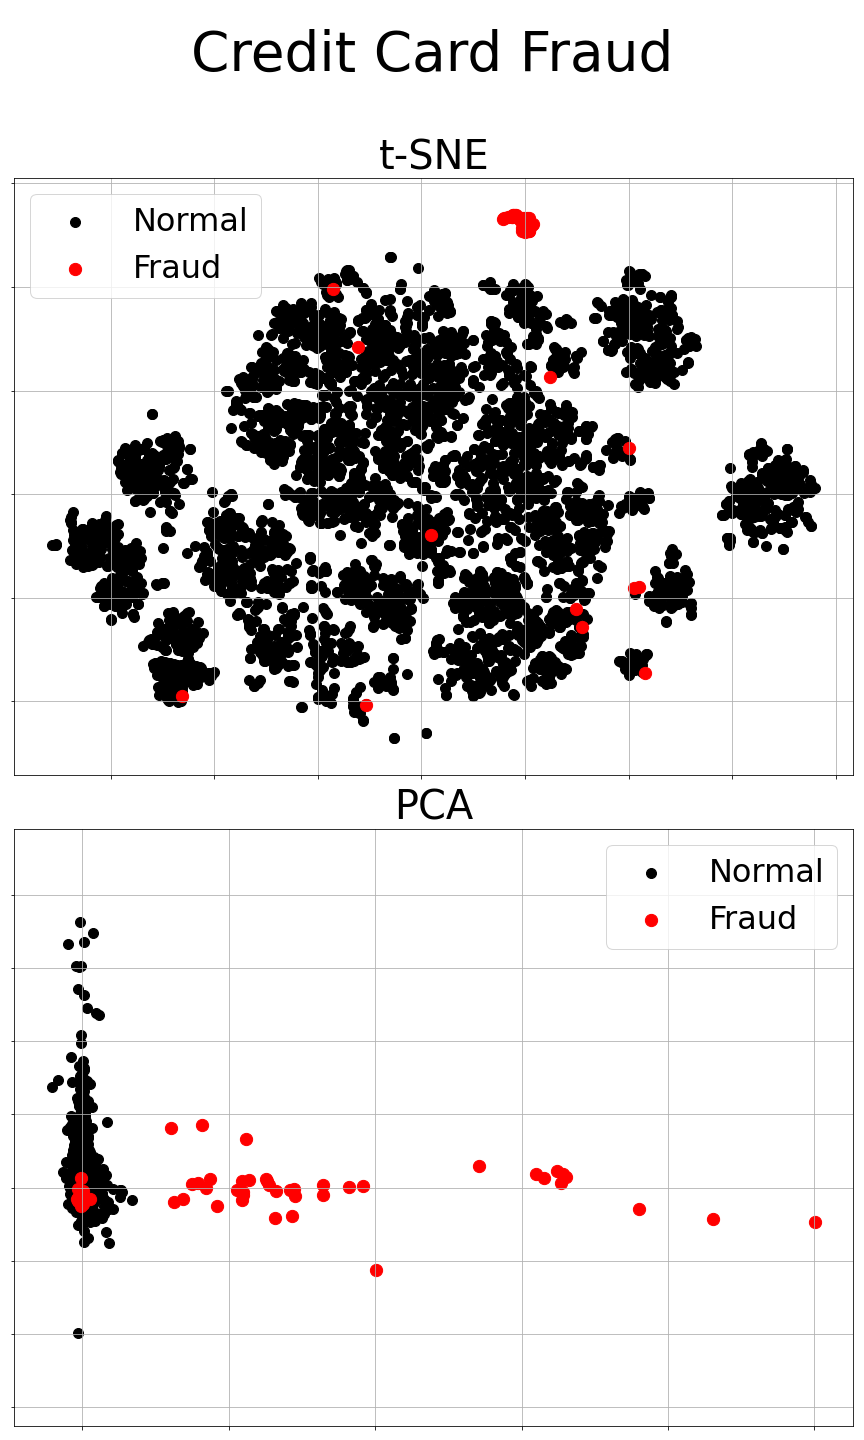
\includegraphics[width=0.283\linewidth]{./images/outlier_figs/OUTLIER_REAL1.png}
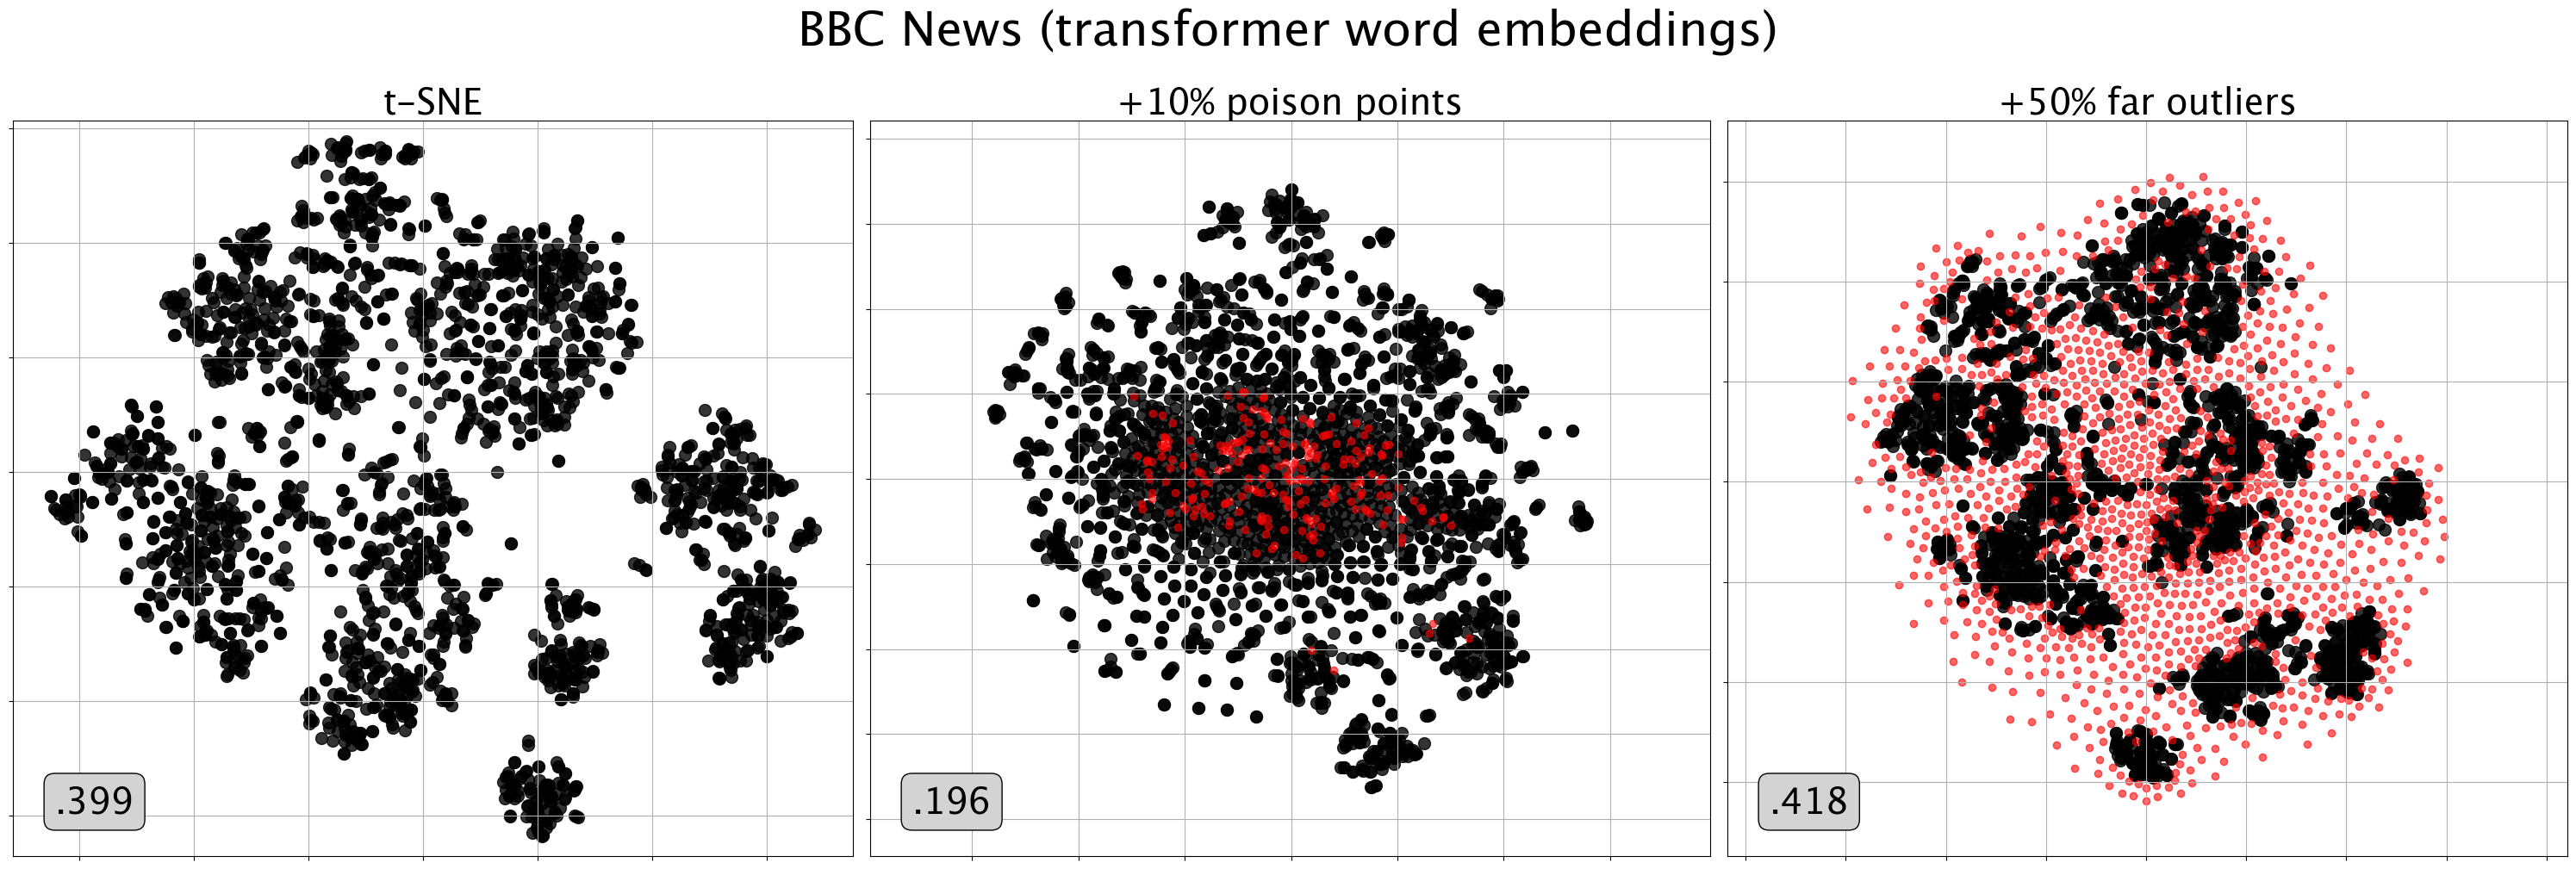
\includegraphics[width=\linewidth]{./images/BBC_POISON.png}
%\vspace{-0.1in}
    \caption{    \small
%\textcolor{red}{FIX CAPTION} 
t-SNE's susceptibility to poison points in contrast with its muted response to outliers, on the BBC news article classification dataset. The bottom left label denotes silhouette score of the original points (without the injected points) with respect to the true labels (business, entertainment, politics, sport, tech).   %Outlier behavior on real-world data. Left: given data monitoring financial activity (\(n=5050\), \(D=30\)) where one percent of users are committing fraud, PCA succeeds and t-SNE fails in visualizing the frauds as outliers. Right: using RoBERTa transformer embeddings of BBC news article titles (\(n=1191, D=768\)), we find that its t-SNE clustering can be destroyed by injecting a relatively small number of ``poison'' points; meanwhile, the clustering structure is remarkably robust to the injection of faraway \((\alpha\gg 1)\)-outliers
}
    \label{fig:outliers_real_world}
%\vspace{-0.1in}
\end{figure}








